\section{Register description}
\regover{
{\hyperref[pds-PDS-CTL]{PDS\_CTL}}&
\\
\hline
{\hyperref[pds-PDS-TIME1]{PDS\_TIME1}}&
\\
\hline
{\hyperref[pds-PDS-INT]{PDS\_INT}}&
\\
\hline
{\hyperref[pds-PDS-CTL2]{PDS\_CTL2}}&
\\
\hline
{\hyperref[pds-PDS-CTL3]{PDS\_CTL3}}&
\\
\hline
{\hyperref[pds-PDS-CTL4]{PDS\_CTL4}}&
\\
\hline
{\hyperref[pds-pds-stat]{pds\_stat}}&
\\
\hline
{\hyperref[pds-pds-ram1]{pds\_ram1}}&
\\
\hline
{\hyperref[pds-PDS-CTL5]{PDS\_CTL5}}&
\\
\hline
{\hyperref[pds-PDS-RAM2]{PDS\_RAM2}}&
\\
\hline
{\hyperref[pds-pds-gpio-i-set]{pds\_gpio\_i\_set}}&
\\
\hline
{\hyperref[pds-pds-gpio-pd-set]{pds\_gpio\_pd\_set}}&
\\
\hline
{\hyperref[pds-pds-gpio-int]{pds\_gpio\_int}}&
\\
\hline
{\hyperref[pds-pds-gpio-stat]{pds\_gpio\_stat}}&
\\
\hline
{\hyperref[pds-PDS-RAM3]{PDS\_RAM3}}&
\\
\hline
{\hyperref[pds-PDS-RAM4]{PDS\_RAM4}}&
\\
\hline
}

\subsection{PDS\_CTL}
\label{pds-PDS-CTL}
Address:0x2000e000
 \begin{figure}[H]
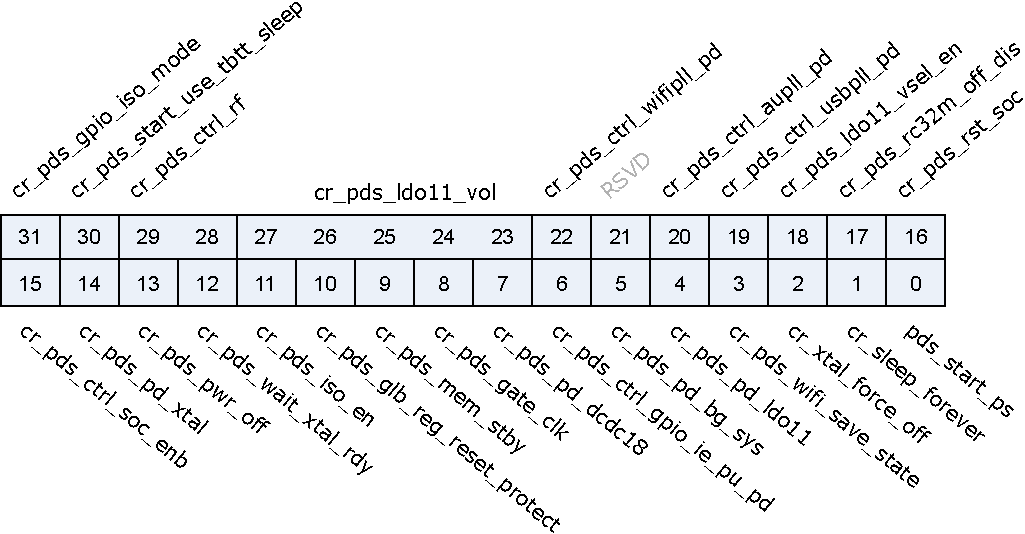
\includegraphics{pds_PDS_CTL.pdf}
\end{figure}

\regdes{31&cr\_pds\_gpio\_iso\_mode&r/w&0&1: HW Keep GPIO  @ PDS7 \par 0 : Clear this bit after PDS7 to release GPIO
\\\hline
30&RSVD& & & \\\hline
29:28&cr\_pds\_ctrl\_rf&r/w&2'b01&00 : PDS don’t control RF on/off \par 01 : PDS control RF on/off depend on misc\_pwr\_off \par 10 : PDS control RF on/off depend on  any power off \par 11 : PDS control RF on/off whe  pds at idle state
\\\hline
27:23&cr\_pds\_ldo11\_vol&r/w&5'h8&LDO11 voltage value in PDS mode \par output voltage sel: 0: 0.9V, 4: 1.0V, 8: 1.1V, 12: 1.2V, 25mV/step
\\\hline
22&cr\_pds\_ctrl\_wifipll\_pd&r/w&0&PDS Control WIFI PLL off When pds\_pwr\_off\\\hline
21&RSVD& & & \\\hline
20&cr\_pds\_ctrl\_aupll\_pd&r/w&0&PDS Control Audio PLL off When pds\_pwr\_off\\\hline
19&cr\_pds\_ctrl\_usbpll\_pd&r/w&0&PDS Control USB PLL off When pds\_pwr\_off\\\hline
18&cr\_pds\_ldo11\_vsel\_en&r/w&0&PDS "SLEEP" control LDO11 voltage enable\\\hline
17&cr\_pds\_rc32m\_off\_dis&r/w&0&1 : RC32M always on  @any state \par 0 : RC32M on/off controlled by PDS state
\\\hline
16&cr\_pds\_rst\_soc&r/w&0&0 : no pds\_reset \par 1: pds\_rst controlled by PDS
\\\hline
15&cr\_pds\_ctrl\_soc\_enb&r/w&0&1 :pds\_soc\_enb controlled by PDS \par 0 :pds\_soc\_enb always active
\\\hline
14&cr\_pds\_pd\_xtal&r/w&1&0 : don’t\_touch xtal  during PDS \par 1 : xtal power down during PDS
\\\hline
13&cr\_pds\_pwr\_off&r/w&1&0 : don’t\_touch Power during PDS    \par 1 : Power off during PDS      (each power domain can has its own control)
\\\hline
12&cr\_pds\_wait\_xtal\_rdy&r/w&0&0 : Skip wait XTAL Ready before  PDS Interrupt \par 1 : wait XTAL Ready during before PDS Interrupt
\\\hline
11&cr\_pds\_iso\_en&r/w&1&0 : don’t\_touch Isolation during PDS (all power domain) \par 1 : Isolation during PDS      (each power domain can has its own control)
\\\hline
10&cr\_pds\_glb\_reg\_reset\_protect&r/w&0&1: avoid glb\_reg reset by any reset\\\hline
9&cr\_pds\_mem\_stby&r/w&1&0 : don’t\_touch mem\_stby during PDS \par 1 : mem\_stby during PDS     (each power domain can has its own control)
\\\hline
8&cr\_pds\_gate\_clk&r/w&1&0 : don’t\_touch clock gating during PDS (all power domain) \par 1 : gate clock during PDS  (each pwr domain has its own control)  
\\\hline
7&cr\_pds\_pd\_dcdc18&r/w&0&0 : don’t\_touch dcdc18 during PDS \par 1 : power down dcdc18 during PDS
\\\hline
6&cr\_pds\_ctrl\_gpio\_ie\_pu\_pd&r/w&0&1: allow PDS Control the GPIO IE/PU/PD at Sleep Mode\\\hline
5&cr\_pds\_pd\_bg\_sys&r/w&0&0 : don’t\_touch bg\_sys during PDS \par 1 : power down bg\_sys during PDS
\\\hline
4&cr\_pds\_pd\_ldo11&r/w&0&0 : don’t\_touch ldo11 during PDS \par 1 : power down ldo11 during PDS
\\\hline
3&cr\_pds\_wifi\_save\_state&r/w&0&Save WIFI State Before Enter PDS\\\hline
2&cr\_xtal\_force\_off&r/w&0&\\\hline
1&cr\_sleep\_forever&r/w&0&\\\hline
0&pds\_start\_ps&w1p&0&Enter PDS\\\hline

}
\subsection{PDS\_TIME1}
\label{pds-PDS-TIME1}
Address:0x2000e004
 \begin{figure}[H]
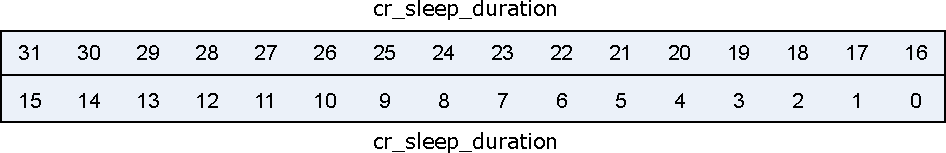
\includegraphics{pds_PDS_TIME1.pdf}
\end{figure}

\regdes{31:0&cr\_sleep\_duration&r/w&32'd3240&PDS Sleep Time (in units of 32K clock cycles)\\\hline

}
\subsection{PDS\_INT}
\label{pds-PDS-INT}
Address:0x2000e00c
 \begin{figure}[H]
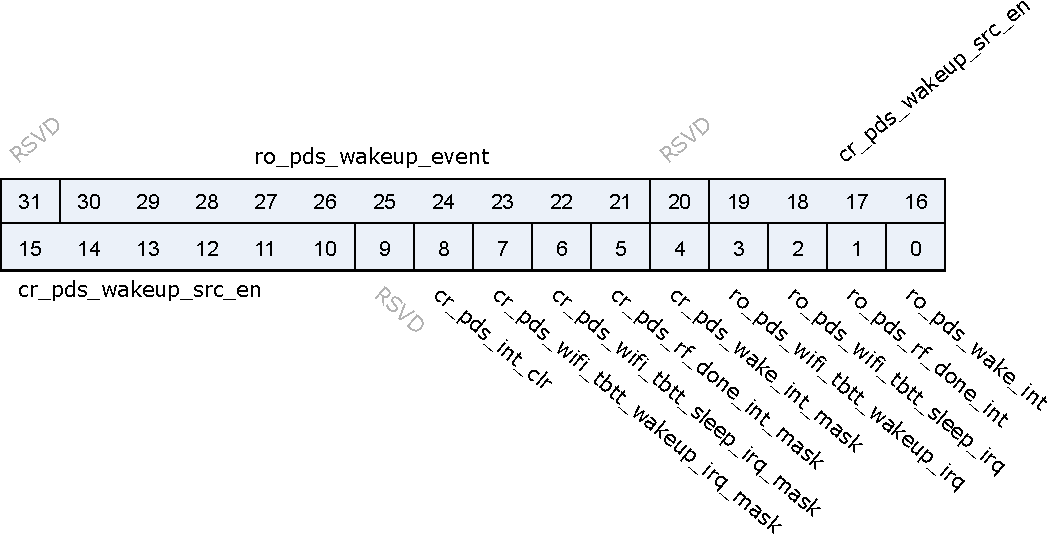
\includegraphics{pds_PDS_INT.pdf}
\end{figure}

\regdes{31:9&RSVD& & & \\\hline
8&cr\_pds\_int\_clr&r/w&0&pds interrupt clear\\\hline
7:6&RSVD& & & \\\hline
5&cr\_pds\_rf\_done\_int\_mask&r/w&0&Mask pds rf done interrupt\\\hline
4&cr\_pds\_wake\_int\_mask&r/w&0&Mask pds wakeup interrupt\\\hline
3:2&RSVD& & & \\\hline
1&ro\_pds\_rf\_done\_int&r&0&pu\_rf\_done interrupt\\\hline
0&ro\_pds\_wake\_int&r&0&PDS Wakeup Interrupt\\\hline

}
\subsection{PDS\_CTL2}
\label{pds-PDS-CTL2}
Address:0x2000e010
 \begin{figure}[H]
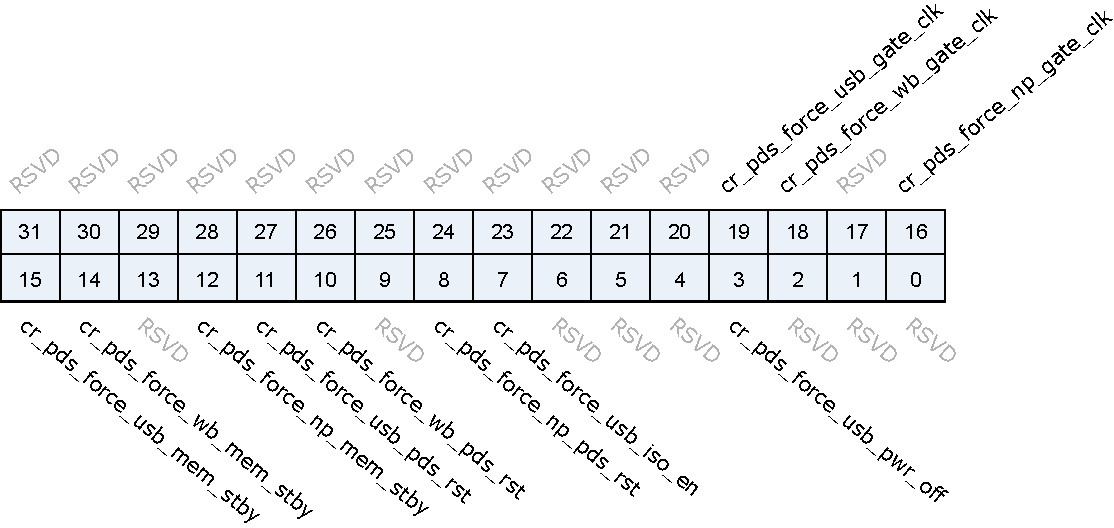
\includegraphics{pds_PDS_CTL2.pdf}
\end{figure}

\regdes{31:20&RSVD& & & \\\hline
19&cr\_pds\_force\_usb\_gate\_clk&r/w&0&manual force usbio clock gated\\\hline
18&cr\_pds\_force\_wb\_gate\_clk&r/w&0&manual force WB clock gated\\\hline
17&RSVD& & & \\\hline
16&cr\_pds\_force\_np\_gate\_clk&r/w&0&manual force NP clock gated\\\hline
15&cr\_pds\_force\_usb\_mem\_stby&r/w&0&manual force usbio memory sleep\\\hline
14&cr\_pds\_force\_wb\_mem\_stby&r/w&0&manual force WB memory sleep\\\hline
13&RSVD& & & \\\hline
12&cr\_pds\_force\_np\_mem\_stby&r/w&0&manual force NP memory sleep\\\hline
11&cr\_pds\_force\_usb\_pds\_rst&r/w&0&manual force usbio pds reset\\\hline
10&cr\_pds\_force\_wb\_pds\_rst&r/w&0&manual force WB pds reset\\\hline
9&RSVD& & & \\\hline
8&cr\_pds\_force\_np\_pds\_rst&r/w&0&manual force NP pds reset\\\hline
7&cr\_pds\_force\_usb\_iso\_en&r/w&0&manual force usbio isolation\\\hline
6&cr\_pds\_force\_wb\_iso\_en&r/w&0&manual force WB isolation\\\hline
5&RSVD& & & \\\hline
4&cr\_pds\_force\_np\_iso\_en&r/w&0&manual force NP isolation\\\hline
3&cr\_pds\_force\_usb\_pwr\_off&r/w&0&manual force usbio power off\\\hline
2&cr\_pds\_force\_wb\_pwr\_off&r/w&0&manual force WB power off\\\hline
1&RSVD& & & \\\hline
0&cr\_pds\_force\_np\_pwr\_off&r/w&0&manual force NP power off\\\hline

}
\subsection{PDS\_CTL3}
\label{pds-PDS-CTL3}
Address:0x2000e014
 \begin{figure}[H]
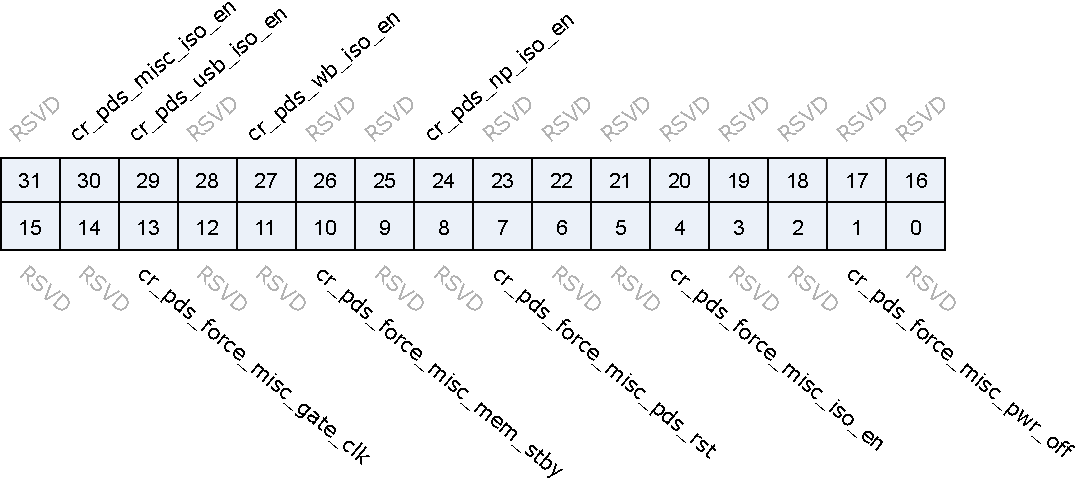
\includegraphics{pds_PDS_CTL3.pdf}
\end{figure}

\regdes{31&RSVD& & & \\\hline
30&cr\_pds\_misc\_iso\_en&r/w&1&1 : make misc isolated at PDS Sleep state \par 0 : make misc isolated at PDS Sleep state
\\\hline
29&cr\_pds\_usb\_iso\_en&r/w&1&1 : make usb isolated at PDS Sleep state \par 0 : make usb isolated at PDS Sleep state
\\\hline
28&RSVD& & & \\\hline
27&cr\_pds\_wb\_iso\_en&r/w&1&1 : make WB isolated at PDS Sleep state \par 0 : make WB isolated at PDS Sleep state
\\\hline
26:25&RSVD& & & \\\hline
24&cr\_pds\_np\_iso\_en&r/w&1&1 : make NP isolated at PDS Sleep state \par 0 : make NP isolated at PDS Sleep state
\\\hline
23:14&RSVD& & & \\\hline
13&cr\_pds\_force\_misc\_gate\_clk&r/w&0&manual force MISC gate\_clk\\\hline
12:11&RSVD& & & \\\hline
10&cr\_pds\_force\_misc\_mem\_stby&r/w&0&manual force MISC mem\_stby\\\hline
9:8&RSVD& & & \\\hline
7&cr\_pds\_force\_misc\_pds\_rst&r/w&0&manual force MISC pds\_rst\\\hline
6:5&RSVD& & & \\\hline
4&cr\_pds\_force\_misc\_iso\_en&r/w&0&manual force MISC iso\_en\\\hline
3:2&RSVD& & & \\\hline
1&cr\_pds\_force\_misc\_pwr\_off&r/w&0&manual force MISC pwr\_off\\\hline
0&RSVD& & & \\\hline

}
\subsection{PDS\_CTL4}
\label{pds-PDS-CTL4}
Address:0x2000e018
 \begin{figure}[H]
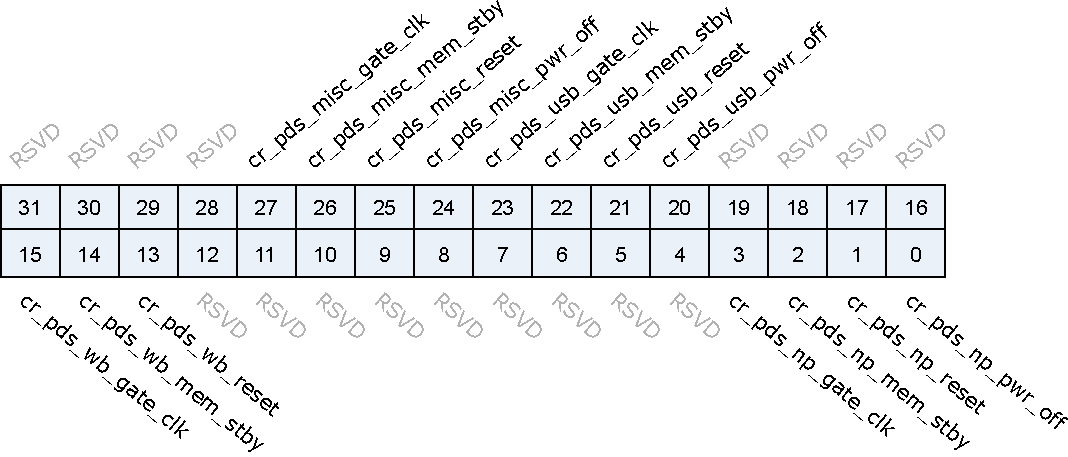
\includegraphics{pds_PDS_CTL4.pdf}
\end{figure}

\regdes{31:28&RSVD& & & \\\hline
27&cr\_pds\_misc\_gate\_clk&r/w&1&1 : make core\_misc clock gated at PDS Sleep state \par 0 : make core\_misc clocking at PDS Sleep state
\\\hline
26&cr\_pds\_misc\_mem\_stby&r/w&1&1 : make core\_misc RAM @Retention at PDS Sleep state \par 0 : make core\_misc RAM @ Normal at PDS Sleep state
\\\hline
25&cr\_pds\_misc\_reset&r/w&1&1 : make core\_misc reset at PDS Sleep state \par 0 : make core\_misc not reset at PDS Sleep state
\\\hline
24&cr\_pds\_misc\_pwr\_off&r/w&1&1 : make core\_misc Power off at PDS Sleep state \par 0 : make core\_misc power on at PDS Sleep state
\\\hline
23&cr\_pds\_usb\_gate\_clk&r/w&1&1 : make usb clock gated at PDS Sleep state \par 0 : make usb clocking at PDS Sleep state
\\\hline
22&cr\_pds\_usb\_mem\_stby&r/w&1&1 : make usb RAM @Retention at PDS Sleep state \par 0 : make usb RAM @ Normal at PDS Sleep state
\\\hline
21&cr\_pds\_usb\_reset&r/w&1&1 : make usb reset at PDS Sleep state \par 0 : make usb not reset at PDS Sleep state
\\\hline
20&cr\_pds\_usb\_pwr\_off&r/w&1&1 : make usb Power off at PDS Sleep state \par 0 : make usb power on at PDS Sleep state
\\\hline
19:16&RSVD& & & \\\hline
15&cr\_pds\_wb\_gate\_clk&r/w&1&1 : make WB clock gated at PDS Sleep state \par 0 : make WB clocking at PDS Sleep state
\\\hline
14&cr\_pds\_wb\_mem\_stby&r/w&1&1 : make WB RAM @Retention at PDS Sleep state \par 0 : make WB RAM @ Normal at PDS Sleep state
\\\hline
13&cr\_pds\_wb\_reset&r/w&1&1 : make WB reset at PDS Sleep state \par 0 : make WB not reset at PDS Sleep state
\\\hline
12&cr\_pds\_wb\_pwr\_off&r/w&1&1 : make WB Power off at PDS Sleep state \par 0 : make WB power on at PDS Sleep state
\\\hline
11:4&RSVD& & & \\\hline
3&cr\_pds\_np\_gate\_clk&r/w&1&1 : make NP clock gated at PDS Sleep state \par 0 : make NP clocking at PDS Sleep state
\\\hline
2&cr\_pds\_np\_mem\_stby&r/w&1&1 : make NP RAM @Retention at PDS Sleep state \par 0 : make NP RAM @ Normal at PDS Sleep state
\\\hline
1&cr\_pds\_np\_reset&r/w&1&1 : make NP reset at PDS Sleep state \par 0 : make NP not reset at PDS Sleep state
\\\hline
0&cr\_pds\_np\_pwr\_off&r/w&1&1 : make NP Power off at PDS Sleep state \par 0 : make NP power on at PDS Sleep state
\\\hline

}
\subsection{pds\_stat}
\label{pds-pds-stat}
Address:0x2000e01c
 \begin{figure}[H]
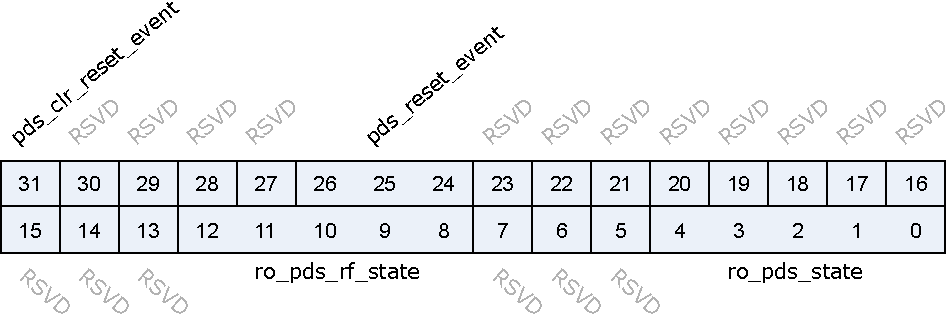
\includegraphics{pds_pds_stat.pdf}
\end{figure}

\regdes{31&pds\_clr\_reset\_event&w1c&0&clear pds reset event\\\hline
30:27&RSVD& & & \\\hline
26:24&pds\_reset\_event&r&0&[2] : pds\_rst\_n (pds reset) \par [1]: pwr\_rst\_n (hbn power on reset) \par [0]: hreset\_n (Bus Reset)
\\\hline
23:13&RSVD& & & \\\hline
12:8&ro\_pds\_rf\_state&r&5'b0&ST\_PDS\_RF\_OFF         = 5'b0000 ; \par ST\_PDS\_PU\_MBG         = 5'b0001 ; \par ST\_PDS\_PU\_LDO15RF = 5'b0011 ; \par ST\_PDS\_PU\_SFREG     = 5'b0111 ; \par ST\_PDS\_PUD\_XTAL18 = 5'b01111; \par ST\_PDS\_WB\_EN\_AON  = 5'b11111 ;
\\\hline
7:5&RSVD& & & \\\hline
4:0&ro\_pds\_state&r&5'b0&ST\_IDLE           = 5'b00000;  \par ST\_MEM\_STBY = 5'b10000;  \par ST\_ECG            = 5'b01000;  \par ST\_ERST          = 5'b01100;  \par ST\_EISO           = 5'b01111;  \par ST\_POFF           = 5'b00111;  \par ST\_PRE\_BGON  = 5'b00011;  \par ST\_PRE\_BGON1 = 5'b00001;  \par ST\_BGON           = 5'b00101;  \par ST\_CLK\_SW\_32M= 5'b00100;  \par ST\_PON\_DCDC    = 5'b00110;  \par ST\_PON\_LDO11\_MISC = 5'b01110;  \par ST\_PON             = 5'b01010;  \par ST\_DISO           = 5'b00010;  \par ST\_DCG            = 5'b01101;  \par ST\_MEM\_IDLE   = 5'b11000;  \par ST\_DRST           = 5'b01011;  \par ST\_WAIT\_EFUSE= 5'b01001;  \par 
\\\hline

}
\subsection{pds\_ram1}
\label{pds-pds-ram1}
Address:0x2000e020
 \begin{figure}[H]
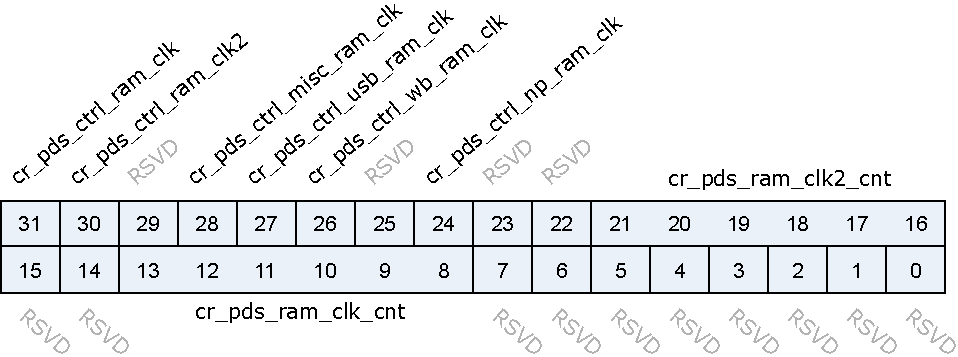
\includegraphics{pds_pds_ram1.pdf}
\end{figure}

\regdes{31&cr\_pds\_ctrl\_ram\_clk&r/w&1'b0&1 : Enable PDS Control PD\_CORE SRAM Clock @ PDS Sequence \par 
\\\hline
30&cr\_pds\_ctrl\_ram\_clk2&r/w&1'b0&HW Option  \par To assert extra clock during PDS on sequence
\\\hline
29&RSVD& & & \\\hline
28&cr\_pds\_ctrl\_misc\_ram\_clk&r/w&1'b0&This bit is Enable by bit [31] : cr\_pds\_ctrl\_ram\_clk \par 1 : PDS Control PD\_CORE\_MISC SRAM Clock @ PDS Sequence \par 0 : PDS do nothing on SRAM Clock
\\\hline
27&cr\_pds\_ctrl\_usb\_ram\_clk&r/w&1'b0&This bit is Enable by bit [31] : cr\_pds\_ctrl\_ram\_clk \par 1 : PDS Control PD\_usb SRAM Clock @ PDS Sequence \par 0 : PDS do nothing on PD\_usb SRAM Clock
\\\hline
26&cr\_pds\_ctrl\_wb\_ram\_clk&r/w&1'b0&This bit is Enable by bit [31] : cr\_pds\_ctrl\_ram\_clk \par 1 : PDS Control PD\_WB SRAM Clock @ PDS Sequence \par 0 : PDS do nothing on PD\_WB SRAM Clock
\\\hline
25&RSVD& & & \\\hline
24&cr\_pds\_ctrl\_np\_ram\_clk&r/w&1'b0&This bit is Enable by bit [31] : cr\_pds\_ctrl\_ram\_clk \par 1 : PDS Control PD\_CORE\_CPU SRAM Clock @ PDS Sequence \par 0 : PDS do nothing on PD\_CORE\_CPU SRAM Clock
\\\hline
23:22&RSVD& & & \\\hline
21:16&cr\_pds\_ram\_clk2\_cnt&r/w&6'd24&HW Option : Assert Extra Clock Counter in MEM\_IDLE\\\hline
15:14&RSVD& & & \\\hline
13:8&cr\_pds\_ram\_clk\_cnt&r/w&6'd8&HW Option : Assert Extra Clock Counter in  MEM\_STBY\\\hline
7:0&RSVD& & & \\\hline

}
\subsection{PDS\_CTL5}
\label{pds-PDS-CTL5}
Address:0x2000e024
 \begin{figure}[H]
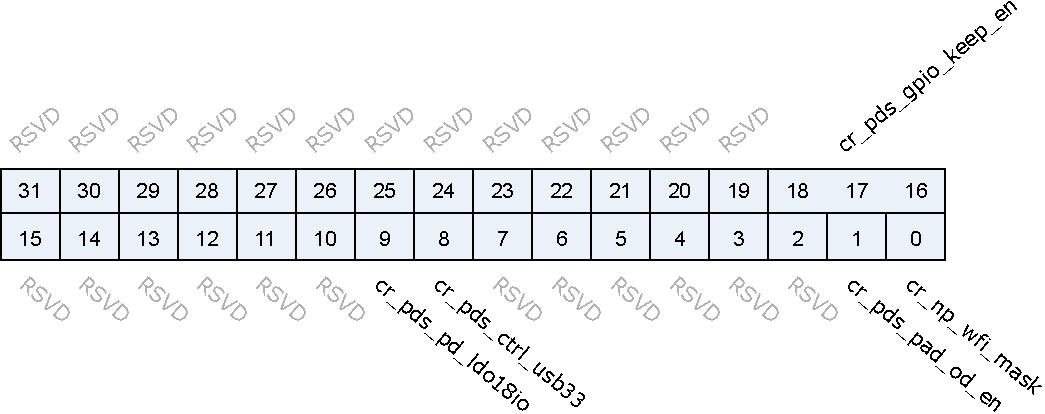
\includegraphics{pds_PDS_CTL5.pdf}
\end{figure}

\regdes{31:19&RSVD& & & \\\hline
18:16&cr\_pds\_gpio\_keep\_en&r/w&3'b111&if cr\_pds\_gpio\_iso\_mode=1, can use bit to enable or disable keep function \par [0] : GPIO0~15 \par [1] : GPIO20~36 (not include GPIO21/22/28/29) \par [2] : GPIO16~19
\\\hline
15:10&RSVD& & & \\\hline
9&cr\_pds\_pd\_ldo18io&r/w&0&0 : don’t\_touch ldo18io during PDS \par 1 : power down ldo18io during PDS
\\\hline
8&cr\_pds\_ctrl\_usb33&r/w&0&Set this bit to enable HW control turn on/off USB 3.3V @USB1.1V Power On/OFF \par (Replace the function of reg\_pu\_usb20\_psw)
\\\hline
7:2&RSVD& & & \\\hline
1&cr\_pds\_pad\_od\_en&r/w&0&GPIO21/22/28/29 5V Tolerant PAD Open Drain Enable\\\hline
0&cr\_np\_wfi\_mask&r/w&0&pds start condition mask np\_wfi\\\hline

}
\subsection{PDS\_RAM2}
\label{pds-PDS-RAM2}
Address:0x2000e028
 \begin{figure}[H]
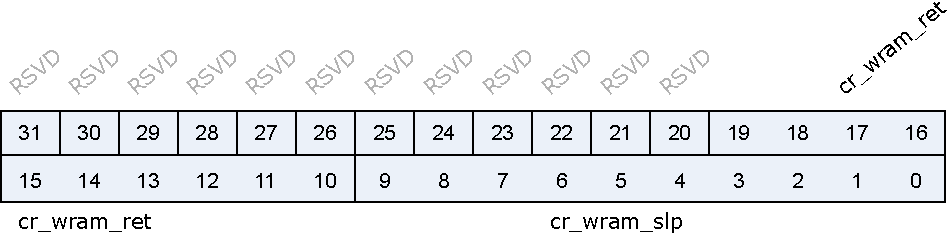
\includegraphics{pds_PDS_RAM2.pdf}
\end{figure}

\regdes{31:20&RSVD& & & \\\hline
19:10&cr\_wram\_ret&r/w&10'h0&[9]    : 144~160KB WRAM Retention \par [8]    : 128~144KB   WRAM Retention \par [7]    : 112~128KB WRAM Retention \par [6]    : 96~112KB WRAM Retention \par [5]    : 80~96KB WRAM Retention \par [4]    : 64~80KB   WRAM Retention \par [3]    : 48~64KB WRAM Retention \par [2]    : 32~48KB WRAM Retention \par [1]    : 16~32KB WRAM Retention \par [0]    : 0~16KB   WRAM Retention
\\\hline
9:0&cr\_wram\_slp&r/w&10'h0&[9]    : 144~160KB WRAM SLEEP \par [8]    : 128~144KB   WRAM SLEEP \par [7]    : 112~128KB WRAM SLEEP \par [6]    : 96~112KB WRAM SLEEP \par [5]    : 80~96KB WRAM SLEEP \par [4]    : 64~80KB   WRAM SLEEP \par [3]    : 48~64KB WRAM SLEEP \par [2]    : 32~48KB WRAM SLEEP \par [1]    : 16~32KB WRAM SLEEP \par [0]    : 0~16KB   WRAM SLEEP
\\\hline

}
\subsection{pds\_gpio\_i\_set}
\label{pds-pds-gpio-i-set}
Address:0x2000e030
 \begin{figure}[H]
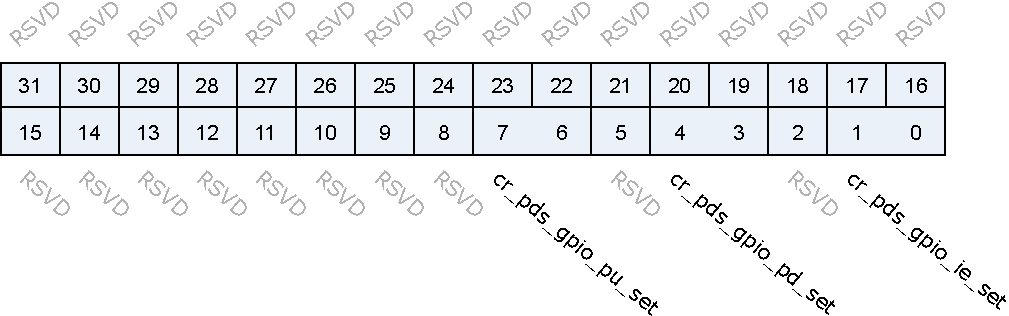
\includegraphics{pds_pds_gpio_i_set.pdf}
\end{figure}

\regdes{31:8&RSVD& & & \\\hline
7:6&cr\_pds\_gpio\_pu\_set&r/w&2'b0&Enable GPIO PU @ PDS \par [0] : GPIO0~15 \par [1] : GPIO20~36
\\\hline
5&RSVD& & & \\\hline
4:3&cr\_pds\_gpio\_pd\_set&r/w&2'b0&Enable GPIO PD @ PDS \par [0] : GPIO0~15 \par [1] : GPIO20~36
\\\hline
2&RSVD& & & \\\hline
1:0&cr\_pds\_gpio\_ie\_set&r/w&2'b0&Enable GPIO IE @ PDS \par [0] : GPIO0~15 \par [1] : GPIO20~36
\\\hline

}
\subsection{pds\_gpio\_pd\_set}
\label{pds-pds-gpio-pd-set}
Address:0x2000e034
 \begin{figure}[H]
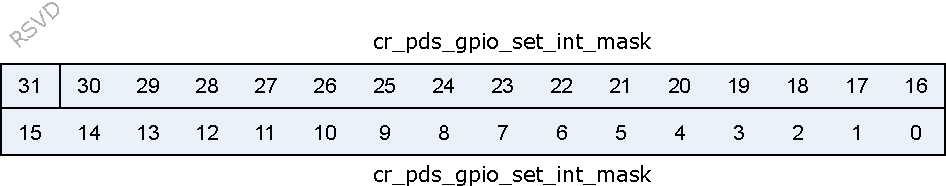
\includegraphics{pds_pds_gpio_pd_set.pdf}
\end{figure}

\regdes{31&RSVD& & & \\\hline
30:0&cr\_pds\_gpio\_set\_int\_mask&r/w&31'h7FFFFFFF&PDS Interrupt Mask for GPIO \par [0] GPIO0 \par [1] GPIO1 \par [2] GPIO2 \par [3] GPIO3 \par [4] GPIO4  \par [5] GPIO5  \par [6] GPIO6  \par [7] GPIO7  \par [8] GPIO8  \par [9] GPIO9  \par [10] GPIO10  \par [11] GPIO11  \par [12] GPIO12  \par [13] GPIO13  \par [14] GPIO14  \par [15] GPIO15  \par [16] GPIO20 \par [17] GPIO21  \par [18] GPIO22  \par [19] GPIO23  \par [20] GPIO24 \par [21] GPIO25  \par [22] GPIO26 \par [23] GPIO27  \par [24] GPIO28  \par [25] GPIO29  \par [26] GPIO30 \par [27] GPIO31 \par [28] GPIO32 \par [29] GPIO33  \par [30] GPIO34  
\\\hline

}
\subsection{pds\_gpio\_int}
\label{pds-pds-gpio-int}
Address:0x2000e040
 \begin{figure}[H]
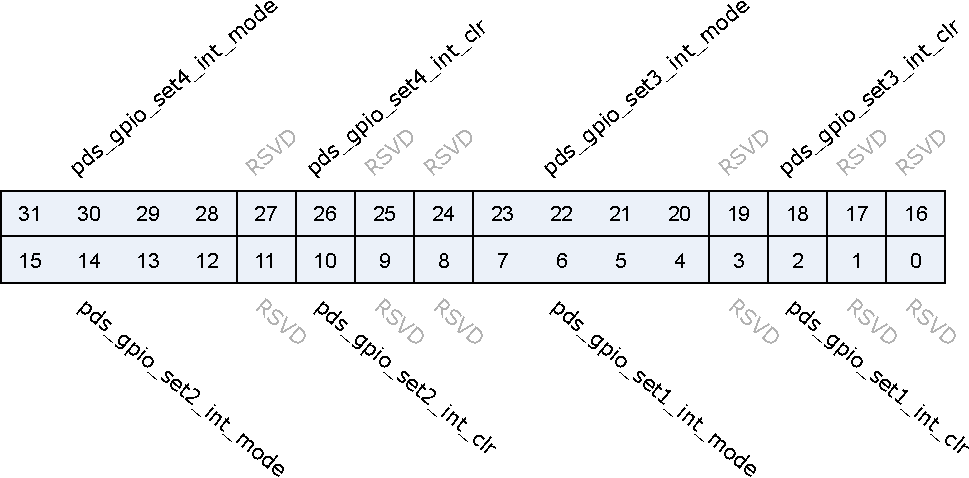
\includegraphics{pds_pds_gpio_int.pdf}
\end{figure}

\regdes{31:28&pds\_gpio\_set4\_int\_mode&r/w&4'b0&GPIO28~34 PDS Interrupt Mode \par 0000 : sync falling edge trigger \par 0001 : sync rising edge trigger \par 0010 : sync low level trigger \par 0011 : sync high level trigger \par 01xx : sync rising \& falling edge trigger \par 1000 : async falling edge trigger \par 1001 : async rising edge trigger \par 1010 : async low level trigger \par 1011 : async high level trigger
\\\hline
27&RSVD& & & \\\hline
26&pds\_gpio\_set4\_int\_clr&r/w&1'b0&Clear GPIO28~34 PDS IO Interrupt\\\hline
25:24&RSVD& & & \\\hline
23:20&pds\_gpio\_set3\_int\_mode&r/w&4'b0&GPIO20~27 PDS Interrupt Mode \par 0000 : sync falling edge trigger \par 0001 : sync rising edge trigger \par 0010 : sync low level trigger \par 0011 : sync high level trigger \par 01xx : sync rising \& falling edge trigger \par 1000 : async falling edge trigger \par 1001 : async rising edge trigger \par 1010 : async low level trigger \par 1011 : async high level trigger
\\\hline
19&RSVD& & & \\\hline
18&pds\_gpio\_set3\_int\_clr&r/w&1'b0&Clear GPIO20~27 PDS IO Interrupt\\\hline
17:16&RSVD& & & \\\hline
15:12&pds\_gpio\_set2\_int\_mode&r/w&4'b0&GPIO8~15  PDS Interrupt Mode \par 0000 : sync falling edge trigger \par 0001 : sync rising edge trigger \par 0010 : sync low level trigger \par 0011 : sync high level trigger \par 01xx : sync rising \& falling edge trigger \par 1000 : async falling edge trigger \par 1001 : async rising edge trigger \par 1010 : async low level trigger \par 1011 : async high level trigger
\\\hline
11&RSVD& & & \\\hline
10&pds\_gpio\_set2\_int\_clr&r/w&1'b0&Clear GPIO8~15  PDS IO Interrupt\\\hline
9:8&RSVD& & & \\\hline
7:4&pds\_gpio\_set1\_int\_mode&r/w&4'b0&GPIO0~7 PDS Interrupt Mode \par 0000 : sync falling edge trigger \par 0001 : sync rising edge trigger \par 0010 : sync low level trigger \par 0011 : sync high level trigger \par 01xx : sync rising \& falling edge trigger \par 1000 : async falling edge trigger \par 1001 : async rising edge trigger \par 1010 : async low level trigger \par 1011 : async high level trigger
\\\hline
3&RSVD& & & \\\hline
2&pds\_gpio\_set1\_int\_clr&r/w&1'b0&Clear GPIO0~7 PDS IO Interrupt\\\hline
1:0&RSVD& & & \\\hline

}
\subsection{pds\_gpio\_stat}
\label{pds-pds-gpio-stat}
Address:0x2000e044
 \begin{figure}[H]
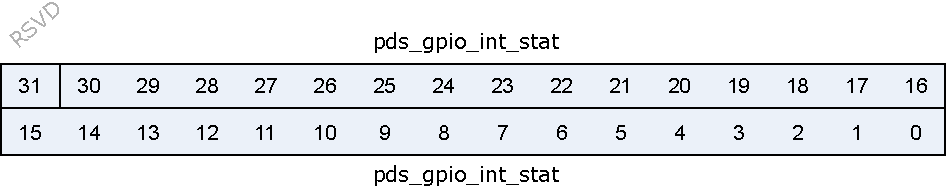
\includegraphics{pds_pds_gpio_stat.pdf}
\end{figure}

\regdes{31&RSVD& & & \\\hline
30:0&pds\_gpio\_int\_stat&r&31'b0&\\\hline

}
\subsection{PDS\_RAM3}
\label{pds-PDS-RAM3}
Address:0x2000e048
 \begin{figure}[H]
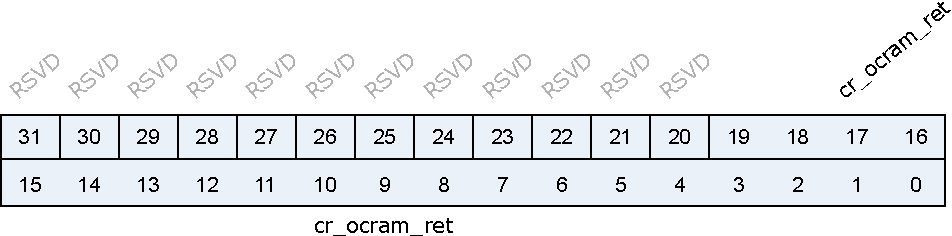
\includegraphics{pds_PDS_RAM3.pdf}
\end{figure}

\regdes{31:20&RSVD& & & \\\hline
19:0&cr\_ocram\_ret&r/w&20'h0&[19]    : 304~320KB OCRAM RET \par [18]    : 288~304KB   OCRAM RET \par [17]    : 272~288KB OCRAM RET \par [16]    : 256~272KB OCRAM RET \par [15]    : 240~256KB OCRAM RET \par [14]    : 224~240KB   OCRAM RET \par [13]    : 208~224KB OCRAM RET \par [12]    : 192~208KB OCRAM RET \par [11]    : 176~192KB OCRAM RET \par [10]    : 160~176KB   OCRAM RET \par [9]    : 144~160KB OCRAM RET \par [8]    : 128~144KB   OCRAM RET \par [7]    : 112~128KB OCRAM RET \par [6]    : 96~112KB OCRAM RET \par [5]    : 80~96KB OCRAM RET \par [4]    : 64~80KB   OCRAM RET \par [3]    : 48~64KB OCRAM RET \par [2]    : 32~48KB OCRAM RET \par [1]    : 16~32KB OCRAM RET \par [0]    : 0~16KB   OCRAM RET
\\\hline

}
\subsection{PDS\_RAM4}
\label{pds-PDS-RAM4}
Address:0x2000e04c
 \begin{figure}[H]
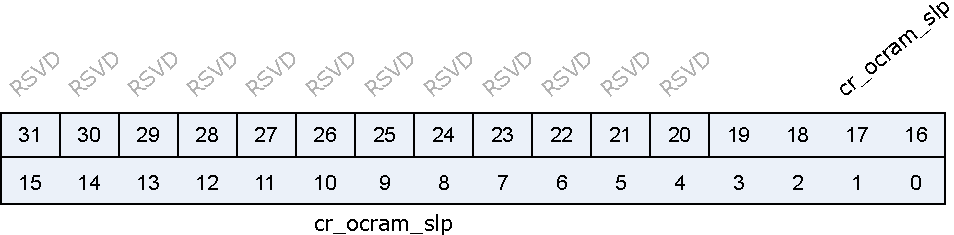
\includegraphics{pds_PDS_RAM4.pdf}
\end{figure}

\regdes{31:20&RSVD& & & \\\hline
19:0&cr\_ocram\_slp&r/w&20'h0&[19]    : 304~320KB OCRAM SLEEP \par [18]    : 288~304KB   OCRAM SLEEP \par [17]    : 272~288KB OCRAM SLEEP \par [16]    : 256~272KB OCRAM SLEEP \par [15]    : 240~256KB OCRAM SLEEP \par [14]    : 224~240KB   OCRAM SLEEP \par [13]    : 208~224KB OCRAM SLEEP \par [12]    : 192~208KB OCRAM SLEEP \par [11]    : 176~192KB OCRAM SLEEP \par [10]    : 160~176KB   OCRAM SLEEP \par [9]    : 144~160KB OCRAM SLEEP \par [8]    : 128~144KB   OCRAM SLEEP \par [7]    : 112~128KB OCRAM SLEEP \par [6]    : 96~112KB OCRAM SLEEP \par [5]    : 80~96KB OCRAM SLEEP \par [4]    : 64~80KB   OCRAM SLEEP \par [3]    : 48~64KB OCRAM SLEEP \par [2]    : 32~48KB OCRAM SLEEP \par [1]    : 16~32KB OCRAM SLEEP \par [0]    : 0~16KB   OCRAM SLEEP
\\\hline

}
